\documentclass[a4paper]{article}


\usepackage[utf8]{inputenc}
\usepackage[T1]{fontenc}
\usepackage{textcomp}
\usepackage{mathtools,amssymb,amsthm}
\usepackage[top=2.5cm,bottom=2.5cm,right=2.5cm,left=2.5cm]{geometry}
\usepackage[francais]{babel}
\usepackage{appendix}

%================image=================
\usepackage{graphicx}
\graphicspath{{figures/}}
\renewcommand{\listfigurename}{Table des figures}

%============header and foot============
\usepackage{fancyhdr}
\pagestyle{fancy}
\renewcommand\headrulewidth{1pt}
\fancyhead[L]{\bfseries POO avec java}
\fancyhead[R]{
\includegraphics[scale=0.05]{./img_rapport/prepisima.png}}
\fancyfoot[L]{CLIQUOT Théo}
\fancyfoot[R]{2020-2021}

% =================other================
\renewcommand{\texttt}[2][blue]{\textcolor{#1}{\ttfamily #2}}
\renewcommand{\contentsname}{Table des matières}
\usepackage{multicol}
%=================code=================
\usepackage{verbatim}
\usepackage{listings}
\usepackage{color}
\usepackage[table]{xcolor}

%==============code settings==========
\definecolor{my_gray}{rgb}{0.20,0.20,0.55}
\definecolor{darkWhite}{rgb}{0.90,0.95,0.90}
\definecolor{myred}{rgb}{1,0.22,0.22}
\definecolor{mypurple}{rgb}{0.74,0.36,0.97}
\lstset{
  mathescape,
  aboveskip=3mm,
  belowskip=-2mm,
  backgroundcolor=\color{darkWhite},
  basicstyle=\ttfamily\footnotesize,
  breakatwhitespace=false,
  breaklines=true,
  captionpos=b,
  commentstyle=\color{myred},
  deletekeywords={...},
  escapeinside={\%*}{*)},
  extendedchars=true,
  framexleftmargin=16pt,
  framextopmargin=3pt,
  framexbottommargin=6pt,
  frame=tb,
  keepspaces=true,
  keywordstyle=\color{mypurple},
  language=C,
  morekeywords={*,...},
  numbers=left,
  numbersep=10pt,
  numberstyle=\tiny\color{black},
  rulecolor=\color{black},
  showspaces=false,
  showstringspaces=false,
  showtabs=false,
  stepnumber=1,
  stringstyle=\color{red},
  tabsize=4,
  title=\lstname,
}

\begin{document}

  \begin{titlepage}
    \begin{center}
  \begin{figure}[!htb]
    \begin{minipage}{0.5\textwidth}
      \centering
      
\includegraphics[width=.7\linewidth]{./img_rapport/prepisima.png}
      \caption{ ISIMA }\label{fig-ISIMA}
    \end{minipage}\hfill
    \begin{minipage}{0.5\textwidth}
      \centering
      
\includegraphics[width=.7\linewidth]{./img_rapport/UCA.jpeg}
      \caption{Université de Clermont-Ferrand}\label{fig-UCA}
    \end{minipage}
  \end{figure}

  \vspace{2cm}



    \color{red}
    {\huge \bfseries TP 5 POO : \\[0.4cm]}
    \color{black}
    \vspace{0.5cm}
    {\huge Réalisation d'équations à l'aide de classe}

    \vspace{4cm}

    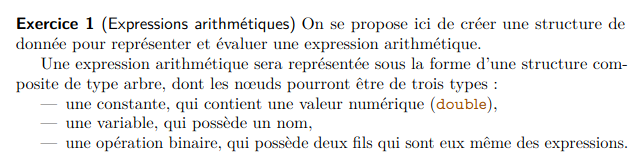
\includegraphics[scale=0.7]{./img_rapport/explic.png}

    \vspace{5cm}
    \color{my_gray}
        CLIQUOT Théo



    \emph{Professeur:} Yannick Loiseau

    Travail à rendre pour le : 1/05/2021
    \color{black}
  \end{center}
\end{titlepage}

\newpage
\begin{center}
  \tableofcontents
  \listoffigures
\end{center}

\newpage
  \section{Division du problème et choix fait}
  \label{sec:div_prob}

  \subsection{Différentes classe}
  \label{subsec:diff_class}


  \begin{multicols}{2}
  Le travail principal demandé est de créer un arbre représentant une équation mathématique, on va donc dans un premier temps devoir créer une classe \texttt{Nœud} qui va accueillir notre valeur à ce nœud mais aussi des fonction que nous verrons plus tard. Cependant chacun de ces nœuds peuvent être divisé en 3 sous nœud différents les uns des autres. Une façon assez intuitive serait donc de créer 3 sous-classe qui vont hériter de \texttt{Nœud} qui seront \texttt{NoeudOperation}, \texttt{NoeudConstante} et \texttt{NoeudVariable} respectivement pour représenter une opération, une constante et une variable. De plus vu qu'on ne va pas instancier d'objet avec la classe \texttt{Nœud}, on peut la rendre {\em abstract}, ce qui permettra en plus de définir des méthodes {\em abstract}. Il n'y aura pas à proprement parlé d'une classe \texttt{Arbre} puisque c'est seulement un \texttt{NoeudOperation} si notre arbre n'est pas composé que d'une racine ou l'un des deux autres sinon. En ce qui concerne le test et l'utilisation du code tout sera dans un fichier à part nommé \texttt{testArbre}.

\end{multicols}

  \subsection{Choix fait}
  \label{subsec:choix_fait}
  \begin{multicols}{2}
    En ce qui concerne les choix faits, j'ai préféré regroupé le plus de fonction possible dans le \texttt{Nœud} afin de simplifier le plus l'utilisation pour l'utilisateur. En effet il n'a pas à se soucier de savoir si son Nœud est une opération, une constante ou une variable lorsqu'il l'utilise, il à sa classe \texttt{Nœud} et c'est tout. Cependant ce n'est pas la classe \texttt{Nœud} qui va contenir l'attribut correspondant à l’élément dans le Nœud car celui-ci peut changer de type en fonction de si il est une constante (Double) ou autre (String) (rien ne nous aurait empêcher de stocker la valeur dans un String pour la constante ou encore de stocker la variable dans \texttt{Nœud} avec comme Type englobant \texttt{Object} mais ça me semblait plus logique dans ce sens). La classe \texttt{Nœud} peut tout de même avoir accès à cette variable avec la méthode \texttt{getValue()}.

    On aurait aussi pu créer une implémentation \texttt{Noeud} et on aurait alors définie chaque Noeud comme l'implémentant mais la première idée qui m'est venue était la classe abstraite englobante.
  \end{multicols}
  
\section{Explication du code}
\label{sec:expli_code}

\subsection{Nœud}
\label{subsec:noeud}

La classe \texttt{Nœud} sera donc abstract et sans attributs. On a aussi surcharger la classe toString qui va juste renvoyer la valeur contenu dans le Nœud en String (évite de le spécifier dans \texttt{NoeudConstante} et \texttt{NoeudVariable}). On aura aussi en méthodes abstraite \texttt{eval()} et \texttt{operation()} qui nous serviront pour la question 3 et enfin une méthode statique \texttt{fromPrefixe()} qui va nous renvoyer l'Arbre (ou le Nœud) correspondant à une expression préfixe. Je l'ai mise dans le Nœud pour 2 raisons :

\vspace{0.5cm}

\begin{itemize}
\item Cela permet de rentrer n'importe quel préfixe et de le transformer en expression, que ce soit une préfixe composé d'opérations comme d'une seule constante. Cependant cela force à regarder la string et en fonction de ce que l'on a d'appeler la méthode \texttt{fromPrefixe()} de la bonne Classe \texttt{Nœud}, mais c'est un choix que j'ai fait comme expliqué là (voir \ref{choix_fait}).

\item On à une séparation de ce problème entre les classes, ce qui rends ce code plus lisible à mon sens avec un effet de yo-yo entre la classe \texttt{Noeud} et la classe \texttt{NoeudOperation}. Cependant si on veut rajouter un nouveau type de nœud on va être obligé de modifier cette méthode. ce qui empêche un peu le côté extensible, mais je ne vois pas d'autre moyen élégant pour rajouter d'autre élément nœud sans perturber la classe \texttt{Nœud}.
  
\end{itemize}

\vspace{0.5cm}

Enfin, on a 2 méthodes privées \texttt{isNumeric()} et \texttt{findIndexParentheseFermante()} qui servent pour notre méthode \texttt{fromPrefixe}. En effet lorsqu'on à le cas d'une opération (c'est à dire un ``(``), on peut se dire qu'on prends le tout et on rappelle la fonction \texttt{fromPrefixe()} récursivement, ce qui va nous faire avancer sans même connaître dans le cas d'une opération en englobant d'autres quand est ce qu'elle finit. Cependant connaître la fin d'une opération permet de diviser de façon plus esthétique et propre le problème à mon sens.

\texttt{isNumeric} va nous permettre de différencier les constantes des variables afin d'appeler la bonne classe. 

\subsection{NoeudConstante}
\label{subsec:noeud_const}

Il n'y a rien de très dur à comprendre avec cette classe, pour \texttt{eval()} tout comme \texttt{getValue()} on retourne le Double stocké dans notre attribut \texttt{val}, si jamais on essaie d'utiliser la méthode \texttt{operation()} on renvoie une erreur car elle ne la supporte pas. Sinon pour le constructeur on va juste appeler le constructeur de la classe mère et initialiser \texttt{val} avec la valeur donné et enfin la méthode statique \texttt{fromPrefixe()} va juste instancier un \texttt{NoeudConstante()} avec comme valeur \texttt{val} celle donné. 


\subsection{NoeudVariable}
\label{subsec:noeud_var}

Très similaire au \texttt{NoeudConstante} (voir \ref{subsec:noeud_const}) avec comme seule différence que la valeur stocké va être du type String et que notre méthode \texttt{eval()} va se servir de la HashMap donnée en argument pour faire correspondre un Double à notre nom de variable. On fait aussi attention que notre nom de variable ne soit pas utilisé pour représenté une opération mais ce n'est pas non plus interdit.

\subsection{NoeudOperation}
\label{subsec:noeud_op}

Le plus gros du travail se fait ici. \texttt{NoeudOperation} n'est qu'une classe abstraite qui va servie comme père pour chaque opération (classe) ; soit :

\vspace{0.5cm}

\begin{itemize}
\item \texttt{NoeudAddition} (voir \ref{subsubsec:noeud_add})
\item \texttt{NoeudSoustraction} (voir \ref{subsubsec:noeud_sub}) 
\item \texttt{NoeudDivision} (voir \ref{subsubsec:noeud_div}) 
\item \texttt{NoeudProduit} (voir \ref{subsubsec:noeud_prod})
\end{itemize}

\begin{multicols}{2}
  
En plus de l'attribut \texttt{val} qui va représenter quelle opération on à dans ce nœud, on aura aussi 2 autres attributs \texttt{Nœud} représentant ce qu'il y a à gauche et à droite de l'opérateur. On va instancier un Nœud operation en se servant du constructeur de \texttt{Nœud} et en initialisant chacun de ses nœuds en attributs à null (rien). Sa méthode \texttt{eval()} va appliquer l’opération a son sous arbre gauche et son sous arbre droit. On aura donc la valeur de l'opération de tous ses nœud enfants et il nous restera plus qu'à faire de même jusqu'à la racine. La méthode \texttt{fromPrefixe()} va continuer sur la même idée mais en sens inverse : On va mettre la valeur de l'opération dans l'attribut \texttt{val} puis on va appeler \texttt{fromPrefixe()} pour obtenir les 2 sous arbres. La méthode \texttt{toString} à été surchargé pour pouvoir afficher non seulement le contenu de \texttt{val} mais aussi celle de ses sous-arbres. Enfin \texttt{creerNoeudOperation()} va seulement appeler la bonne sous classe en fonction de l'opération.
\end{multicols}


\subsubsection{NoeudAddition}
\label{subsubsec:noeud_add}

Les 4 classe qui suivent se ressemblent beaucoup, la seule différence est comment va être gérés la méthode \texttt{opération()} et la valeur stocké dans l'attribut \texttt{val} de \texttt{NoeudOperation}, pour celle ci se sera l'addition et ``+'';

\subsubsection{NoeudSoustraction}
\label{subsubsec:noeud_sub}

La méthode \texttt{operation()} va renvoyer la soustraction de l'élément gauche avec le droit et on va stocker ``-'' dans \texttt{val}. 

\subsubsection{NoeudDivision}
\label{subsubsec:noeud_div}

La méthode \texttt{operation()} va renvoyer la division de l'élément gauche avec le droit et on va stocker ``/''  dans \texttt{val}. 

\subsubsection{NoeudProduit}
\label{subsubsec:noeud_prod}

La méthode \texttt{operation()} va renvoyer le produit de l'élément gauche avec le droit et on va stocker ``*'' dans \texttt{val}. 


\section{Main (test)}
\label{test}

C'est juste un main pour appeler et tester les différentes fonctions, une fois lancé on à un exemple et ensuite on peut le tester nous même en rentrant l'expression en préfixe ainsi que l'ensemble de nos variables (à noter qu'on transforme les ',' en '.' est ce pour prendre en compte la notation française ou anglaise de la virgule).

\begin{lstlisting}
mot = mot.replace(',','.');
\end{lstlisting}

\section{Conclusion}

Ce compte rendu explique brièvement le code et se concentre surtout sur mes choix pour résoudre ce problème car il n'existe pas une seule et unique façon d'implémenter un arbre. Une Javadoc et des commentaires sont présent dans les programmes pour expliquer ce que fait chaque méthodes.

\end{document}